\documentclass{report}
\usepackage{graphicx}
\usepackage{setspace}
\usepackage[margin=1in]{geometry}
\usepackage[dvipsnames]{xcolor}
\usepackage{hyperref}
\usepackage{listings}

\linespread{1.5}

\lstdefinelanguage{SQL}{
	keywords = {,SELECT ,FROM,JOIN,WHERE, GROUP BY, UPDATE, INTO,INSERT, delete, if, end if, else, declare, case, when, connect, prior, start, with, end, as, then, join, union, all, order, siblings, by, desc, IS, NULL, NOT, },
	sensitive=false,
	keywordstyle = \color{blue},
	ndkeywords={,utbc_agreements,utbc_contract,utbc_document,utbc_email, utbc_department,utbc_vendor,utbc_former_name,utbc_tickler, utbc_approvals,utbc_agree_app,utbc_triggers,utbc_agree_trig,},
	ndkeywordstyle = \color{OliveGreen},
	sensitive=false,
	morecomment=[l]{--},
	commentstyle=\color{purple}\ttfamily,
	stringstyle = \ttfamily
	}
	
\lstset{
	language = SQL,
	extendedchars = true,
	basicstyle = \color{red}\ttfamily,
	numbers = left,
	numberstyle=\color{black},
	frame = leftline,
	linecolor=black,
	rulecolor=\color{black}
	}
	
	
\begin{document}

\title{\bfseries UT Business Contracts Application Documentation}

\author{
	Colin Murray (Team Leader)
	\and
	Calvin Aisenbrey
	\and
	Alex Landaverde
	\and
	Chris Metcalf
	\and
	Ashley Ng
}

\maketitle

\begin{abstract}
Put abstract here
\end{abstract}

\tableofcontents

\newpage

\begin{image}
\centering
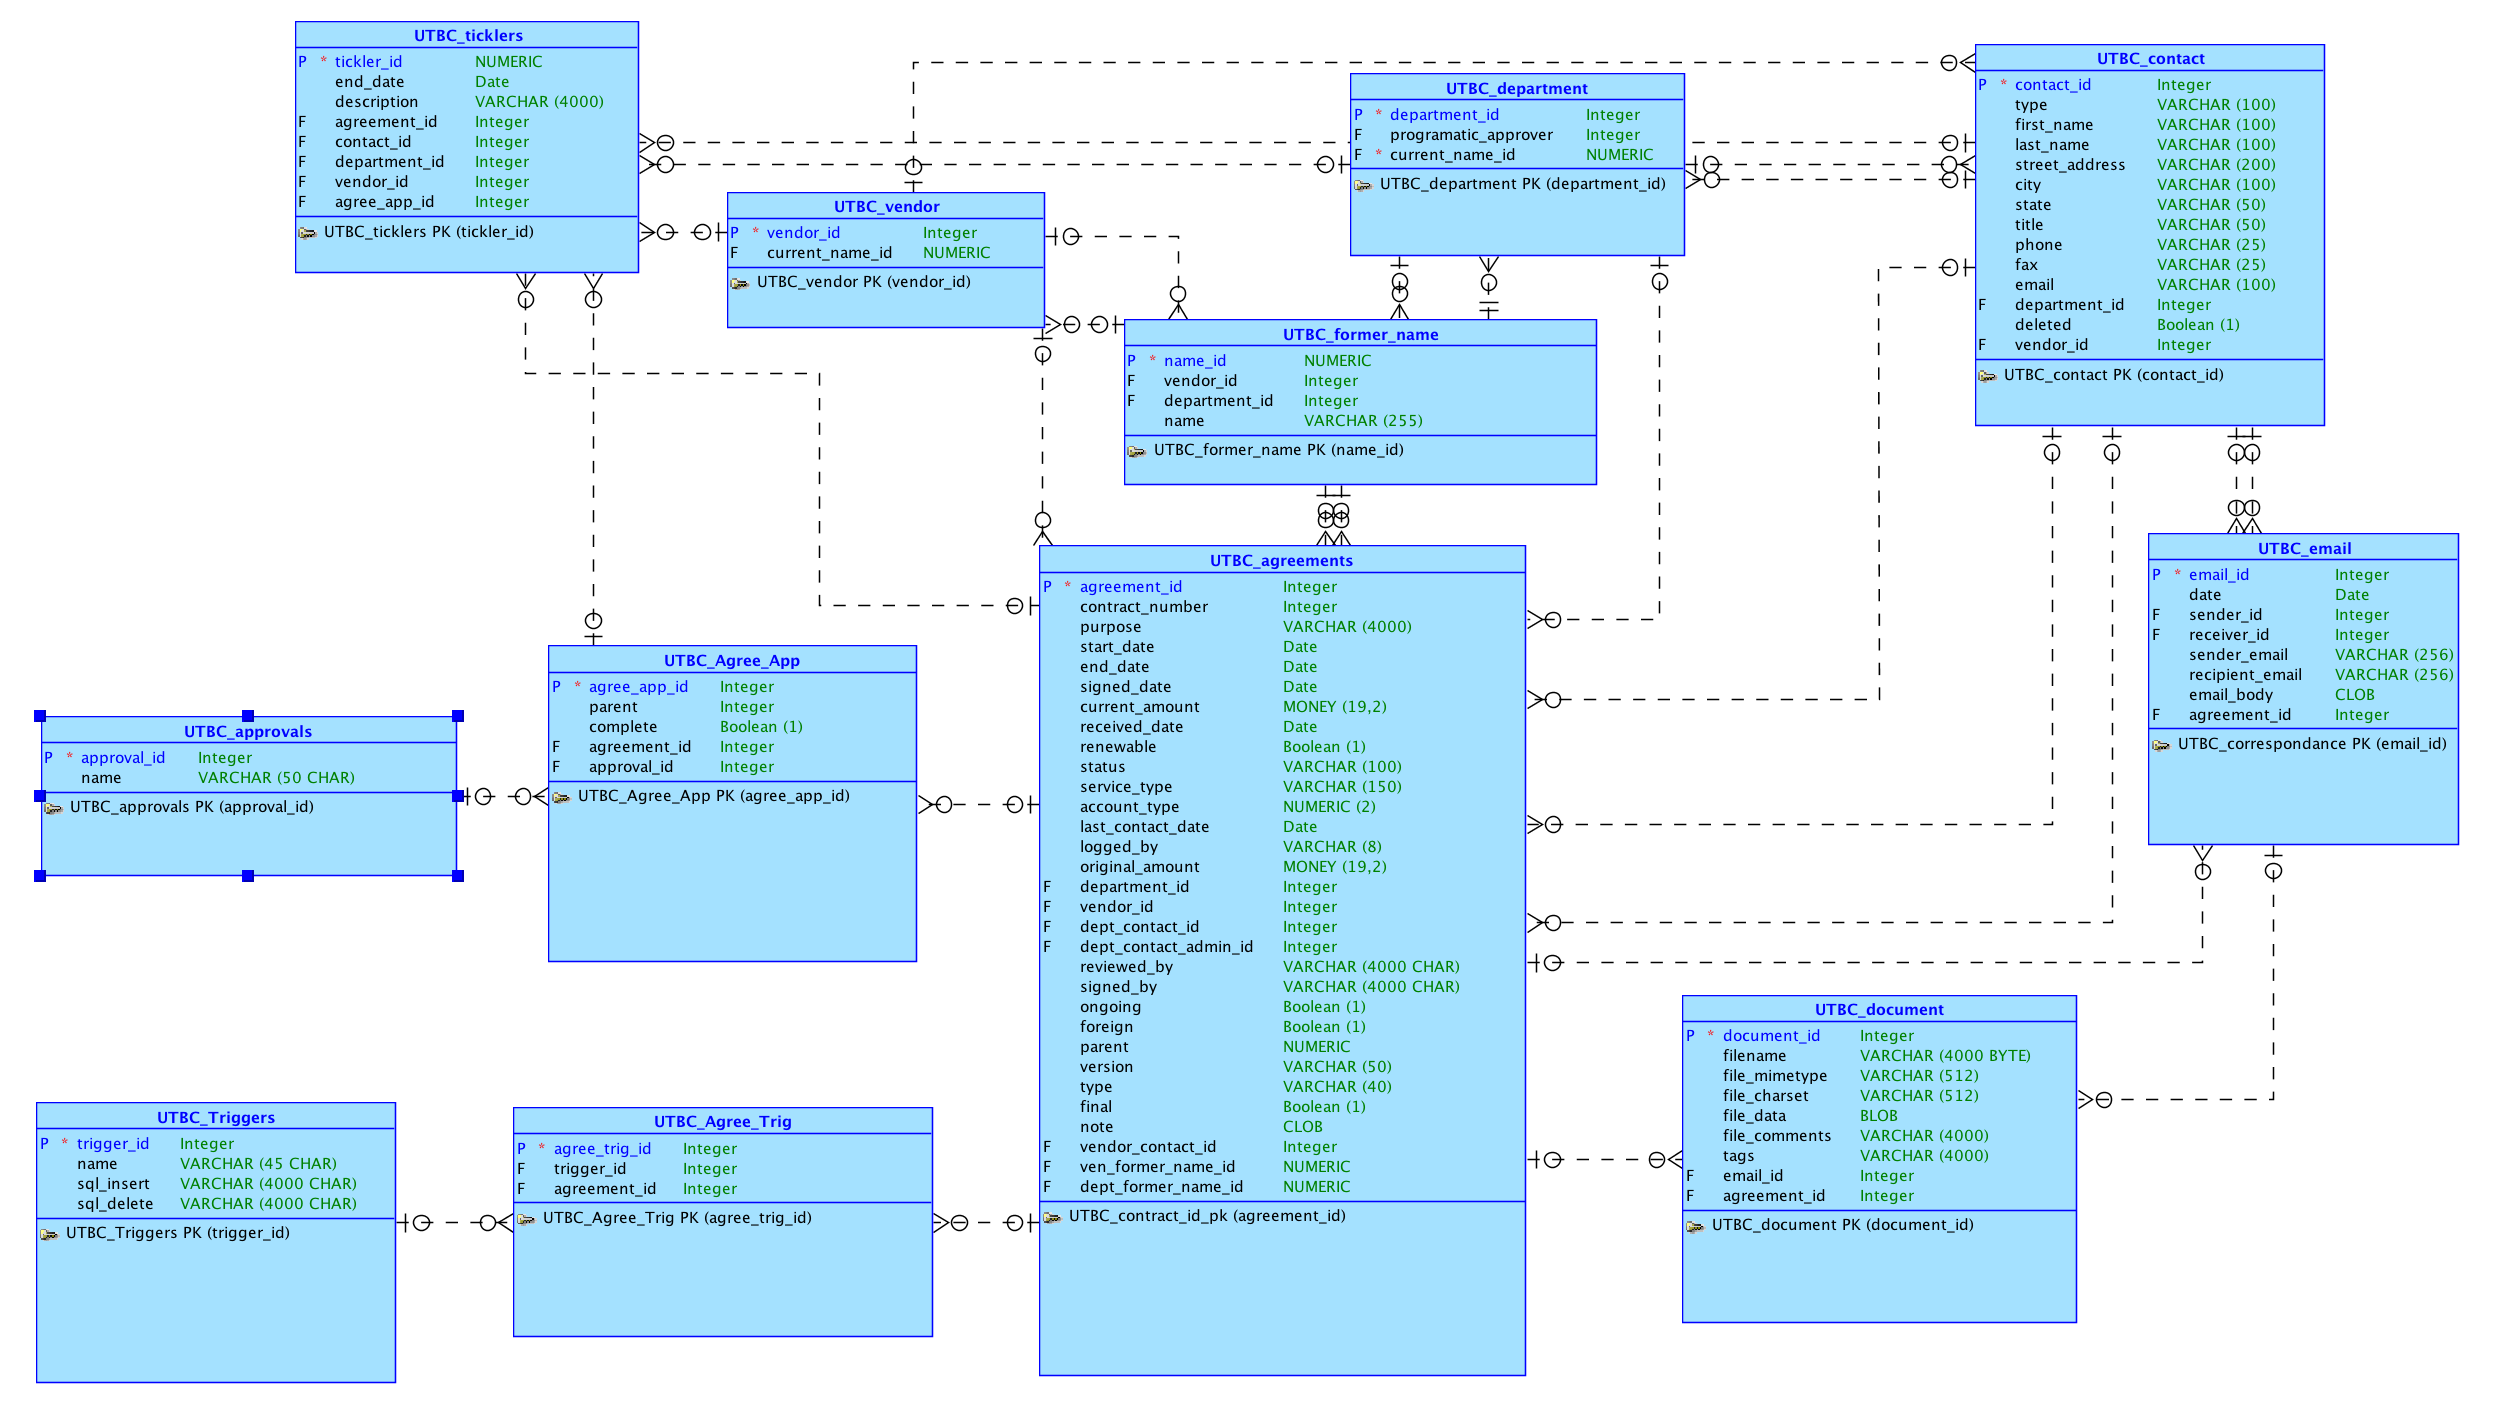
\includegraphics[height = 4.5in, angle = 90]{UTBC_model}
\end{image}



\chapter{Data model}

\section{Contract Table}

\section{UTBC\_approvals and UTBC\_Agree\_App Tables}
The UTBC\_approvals table stores the name of type of approvals. An example of one row would be 3 Informal Quotes. It has a one-to-many relationship with UTBC\_Agree\_App, this was done to simulate a many-to-many relationship from UTBC\_approvals to UTBC\_agreements. By having the UTBC\_Agree\_App, more information can be stored as attributes (parent integer, complete boolean). The parent and complete attribute, helps keep a sense of hierarchy of the approvals that still need to be completed. 

\section{UTBC\_triggers and UTBC\_Agree\_Trig Tables}
The UTBC\_triggers table stores the trigger words (ie  >25k, computer access, etc) which need a certain set of approvals. In the table there are two VARCHAR attributes named sql\_insert and sql\_delete. As the name suggest the attribute contains names to procedures which either insert or delete rows from the UTBC\_Agree\_App table which are executed by a trigger. The UTBC\_triggers has a one-to-many relationship to UTBC\_Agree\_Trig table which it has a many-to-one relationship to UTBC\_Agreements. This was done to simulate a many-to-many relationship from UTBC\_triggers to UTBC\_Agreements. 

\chapter{Application}

\section{Home Page}
The home page consists of three different tables; contracts, ticklers, and BOR dates. The tables only displays contracts that are renewable and are expiring in the next 60 days. The table also only displays contracts that pertain to the user logged in using the where clause

\begin{lstlisting}[caption=Contracts table where clause for user]
WHERE reviewed_by APEX_UTIL.GET_SESSION_STATE('APP_USER')
\end{lstlisting}

The next table is ticklers (or reminders), which only displays ticklers pertaining to the user that is logged in as well as public ticklers for everyone to see. We used the following where clause to do this

\begin{lstlisting}[caption=Tickler table where clause]
WHERE t.created_by = APEX_UTIL.GET_SESSION_STATE('APP_USER')
OR PUBLIC_T = 'Y'
\end{lstlisting}

In this ticklers table, two tables are joined; the UTBC\_ticklers and UTBC\_contact tables. That way the user can easily email the corresponding person about the tickler. 
The next table is BOR dates (or board of regents dates). This table has no connect do our data model and is a stand alone table. The table has two attributes, due date and meeting date. The due date is the day the office will have to get certain paperwork submitted to be on the associated meeting date.

\section{Agreements Home Page}

\subsection{Agreements Tree}
The tree on the Agreements page is created by selecting a set of columns (status, level, title, icon, value, tooltip and link) from a table constructed from a series of unions.

\begin{lstlisting}[caption=Agreement tree select statement]
select case when connect_by_isleaf = 1 then 0
            when level = 1             then 1
            else                           -1
       end as status, 
       level,
       label||to_char(name) as title, 
       case when item_type = 'C' then 
       '#IMAGE_PREFIX#menu/blue_function_16x16.gif' 
            when item_type = 'A' then 
            '#IMAGE_PREFIX#menu/jtfunexe_16x16.gif'
            when item_type = 'V' then 
            '#IMAGE_PREFIX#menu/blue_folder_16x16.gif'
            when item_type = 'VE' then 
            '#IMAGE_PREFIX#menu/hs_infohidden_16x16.gif'
       else null
       end as icon, 
       id as value, 
       case when tooltip is not null then name ||' - '||tooltip
            else name
       end as tooltip,
       case when item_type = 'C' then 
               apex_util.prepare_url(
               'f?p='||:app_id||':4:'||:app_session||':T::4:P7_TREE_NODE,
               P4_AGREEMENT_ID:'||id||','||id)
            when item_type = 'A' then
               apex_util.prepare_url(
               'f?p='||:app_id||':4:'||:app_session||':T::4:P7_TREE_NODE,
               P4_AGREEMENT_ID:'||id||','||id)
            when item_type = 'VE' then 
               apex_util.prepare_url(
               'f?p='||:app_id||':4:'||:app_session||':T::4:P7_TREE_NODE,
               P4_AGREEMENT_ID:'||id||','||id)
       end as link 
 from ( ...
\end{lstlisting}

The primary things to note are:
\begin{itemize}
	\item The name of each node entry on the tree is derived from the 'title' column which is composed of the 'label' appended with the 'name' columns.
  \item The icon is selected depending on the value within the item\_type column.
  \item The link column specifies where the page navigates when a node is clicked.  It is also dependent on the value in the item\_type column.  There is no link for when item\_type = 'V' as there is with icon because items of this type represent the version folder which will be discussed later.  The version folder has no link since it does not represent a real database item.
\end{itemize}
The sql after the from clause constructs a table from a series of unions.  Each union is between the UTBC\_agreements table and itself, but with different rows being selected.  Each union also gets all the rows for one of the 4 item\_types: 

\begin{itemize}
	\item C  (for base contract)
	\item A  (for any sub-agreement like an amendment)
	\item V  (for the version folder)
	\item VE (for all versions of a particular contract or sub-agreement).
\end{itemize}

\begin{lstlisting}[caption=Selecting the max version of each contract in the agreements table.]
--Top of the tree, populated with max versions of each contract.  
--Agreement parent is null.  Links only to the max version for this contract
SELECT 'C' item_type,
       a.type||': ' label,
       a.AGREEMENT_ID id,
       --children of this contract should have 
       --their parent column match this tree_id
       to_char(a.version_parent)||'-'||a.type tree_id,
       --parent should be null
       null parent,
       --constructs the displayed name for a contract in the tree
       to_char(a.contract_number) || ' | ' || (
       select name from UTBC_vendor where vendor_id = a.vendor_id) || ' | ' ||
          (select name from UTBC_department 
          where department_id = a.department_id)
           || ' | ' || to_char(a.start_date, 'MM/DD/YYYY') name, 
       t.tooltip tooltip,
       null link,
       a.DATE_ACCESSED
  FROM UTBC_agreements a, (
  SELECT wwv_flow_lang.system_message('Contract tooltip placeholder') 
  tooltip FROM dual) t
  WHERE a.agreement_parent IS null AND a.version = (
  SELECT MAX(version) FROM UTBC_agreements 
  WHERE version_parent = a.version_parent) and ROWNUM <= :P7_ROW_NUM
\end{lstlisting}

The item\_type column in this select is set to 'C'.  The 'label' column is simply the type column in the agreements table.  In this case that type should be the string 'Contract'.  The 'id' is populated with the agreement\_id of each contract chosen by the select.  The 'name' column is constructed by appending the contract\_number, vendor name, department name and start\_date columns together.  The date\_accessed column is used for sorting.  The most important aspect is the 'parent' and 'tree\_id' columns.

\begin{itemize}
	\item 'tree\_id' specifies the unique identifier that will associate this item with all of it's children.  It is the 'version\_parent' column appended with the type (which is 'Contract').  The version\_parent column will be shared between all versions of this contract, so any child of this contract (say a sub-agreement) can be seen as a child of the version\_parent (which is the agreement\_id of version 0 for all entries in the agreements table).
	\item 'parent' specifies the 'tree\_id' this entry will become a child of.  Since this first select represents the top of the tree, the parent column is left null.
\end{itemize}

!!The tooltip is currently a placeholder chosen from dual, but will change later.
The WHERE clause first makes sure the agreement\_parent column for this agreement is NULL.  All contracts have a null agreement\_parent since they are not sub-agreements.  It next specifies the version column should be the max version for this particular contract.  This can be done by finding the max for all rows that have the same version\_parent column, since only versions of the same agreement share a version\_parent.  Finally, the number of top-level rows displayed depends on the ROWNUM being less than :P7\_ROW\_NUM, an LOV item on the page which allows 10, 50 and 100 recently viewed contracts to be shown at one time.

\begin{lstlisting}[caption=Select statement grabbing all sub-agreements and piling them under their parent contracts.]
UNION ALL
--Gets all sub-agreements (anything with a non-null agreement_parent column).  Links only to the max version for this sub-agreement
SELECT 'A' item_type,
       b.type||': ' label,
       b.agreement_id id,
       --tree id should have the form (version_parent)-(sub-agreement type)
       to_char(b.version_parent)||'-'||b.type tree_id,
       --these should only match up with the 
       --agreement_id their parent contracts
       to_char(b.agreement_parent)||'-Contract' parent,
       --display name for a sub-agreement in the tree
       to_char(b.contract_number) || ' - ' || 
       to_char(b.start_date, 'MM/DD/YYYY')  name,
       u.tooltip tooltip,
       b.DATE_ACCESSED,
       null link
  FROM UTBC_agreements b, (
  	SELECT wwv_flow_lang.system_message
		('Sub-agreement tooltip placeholder') tooltip FROM dual) u
  WHERE b.version = (
  	SELECT MAX(version) 
	FROM UTBC_agreements 
	WHERE version_parent = b.version_parent) 
	AND b.agreement_parent IS NOT null
\end{lstlisting}
This select statement grabs all sub-agreements and associates them as children in the tree to their parent contracts.  The item\_type column is 'A' (standing for Amendment, though they could be any type of sub-agreement).  Many of the columns are otherwise very similar with the exception of tree\_id and parent.

\begin{itemize}
	\item 'tree\_id' will carries the main distinction that b.type will never be 'Contract'.  This allows a way to distinguish whether a version entry in the tree should fall under a contract or a sub-agreement.
	\item 'parent' is created by appending the agreement\_parent with the string '-Contract'.  This hard-codes sub-agreements to always fall under entries that are of type 'Contract'.  The agreement\_parent will always match the version\_parent column for the parent contract, each referring to the agreement\_id of version 0.
\end{itemize}

The where clause selects only agreements where the agreement\_parent column is NOT NULL (meaning it is a sub-agreement) and where the row selected is the max version for this particular sub-agreement (this is done the same way it is done for contracts explained earlier).

\begin{lstlisting}[caption=Select statement creating a dummy version folder entry in the tree.]
--Dummy selection used to create a versions 
--folder to store all the versions for an agreement in
SELECT 'V' item_type,
       'Versions' label,
       c.AGREEMENT_ID id,
       to_char(c.version_parent)||'-'||c.type||'-v' tree_id,
       to_char(c.version_parent)||'-'||c.type parent,--(
       	select type from utbc_agreements where agreement_id = c.parent) parent,
       null name,
       w.tooltip tooltip,
       c.DATE_ACCESSED,
       null link
  FROM UTBC_agreements c, (
  	SELECT wwv_flow_lang.system_message
		('Version folder tooltip placeholder') 
		tooltip FROM dual) w
  WHERE c.version = 0
\end{lstlisting}

The select statement above is of item\_type 'V'.  It creates all the version folders in the tree.  Every contract or sub\_agreement node in the tree should have a version folder as a child node.  To achieve this, the version folder actually represents version 0 of the associated agreement.  Since all contracts or sub-agreements have exactly one version 0, all entries in the tree will receive a version folder.

\begin{itemize}
	\item 'tree\_id' in this case is the version\_parent column, concatenated with the type of agreement, concatenated with '-v'.  The '-v' at the end distinguishes this entry as the version folder and will be used in the 4th union to pile all version entries under this tree-id.
	\item 'parent' operates the same as it would with sub-agreements, except version\_parent is used instead of agreement\_parent.
\end{itemize}

\begin{lstlisting}[caption=Select statement getting all versions for a particular contract and making them children of the version folder.]
UNION ALL
--versions selected here will fall under the version folder
SELECT 'VE' item_type,
       'Version: ' label,
       e.AGREEMENT_ID id,
       to_char(e.AGREEMENT_ID) || '-version' tree_id,
       to_char(e.version_parent)||'-'||e.type||'-v' parent,
       to_char(e.version) name,
       x.tooltip tooltip,
       null link,
       e.DATE_ACCESSED
  FROM UTBC_agreements e, (
  SELECT wwv_flow_lang.system_message
  	('Version tooltip placeholder') 
	tooltip FROM dual) x
\end{lstlisting}

The item\_type for this last union is 'VE'.  The main items to note are the tree\_id and parent:

\begin{itemize}
	\item 'tree\_id' is simply the agreement\_id for this version concatenated with an indicator, specifying that this tree entry is a version.  Since version's have no children, this is unused as of yet.
	\item 'parent' binds all versions of a particular contract as children of the appropriate version folder.  It is constructed in the exact same way 'tree\_id' is created for the version folder entries, meaning even version 0 (which is exploited to create the version folder) is a child of the version folder.  This also demonstrates why version 0 is a child of its self (in terms of version\_parent).
\end{itemize}

There is no where clause since every item in the agreements table is a version of something.

\begin{lstlisting}[caption=final pieces of the initial select statement creating the tree structure.]
)
START WITH parent IS null
CONNECT BY PRIOR tree_id = parent
order siblings by DATE_ACCESSED desc, name
\end{lstlisting}

This statement comes after the from ( ... unions ... ) clause and is responsible for building the tree structure.  It suggests that the first entries in the tree are ones with a NULL parent column.  That child entries are associated with parent entries if the parent's 'tree\_id' matches the child's 'parent' columns.  Finally, all entries in the tree are ordered by the date an agreement was most recently viewed first, then the name second.

\subsection{Agreements Search Bar}
Colin 

\subsection{Agreements Sorting}
The agreements are sorted by showing the agreements which were accessed the most recent at the top of the tree and with agreements accessed the least recent at the bottom. This was accomplished by adding a DATE\_ACCESSED attribute to all of the sub-queries in the tree. At the end of the query the tree is ordered by DATE\_ACCESSED and then alphabetically by name. 

\subsection{Agreements Form}
The agreements form is made as a normal page because of the amount of information and foreign keys you could add from the agreements page. Such as adding new departments, department contacts, department administrator, and vendors from the agreements form. The contract number is assigned from a trigger and sequence

\begin{lstlisting}[caption=Agreement table PK trigger]
create or replace trigger UTBC_agreements_PK_trig 
before insert on UTBC_agreements
for each row 
declare
	type version_table IS TABLE OF UTBC_agreements.version%type;
	t_version version_table;
begin 
	select UTBC_agreements_seq.nextval into :new.agreement_id from dual;
	IF :NEW.CONTRACT_NUMBER is NULL THEN
		select UTBC_CONTRACT_NUMBER_SEQ.nextval 
		into :NEW.CONTRACT_NUMBER from dual;
	END IF;
	IF :NEW.VERSION_PARENT is NULL THEN
		:NEW.VERSION_PARENT := :NEW.AGREEMENT_ID;
	END IF;
	IF :NEW.VERSION is NULL THEN
		select 0 into :NEW.VERSION from dual;
	ELSE 
  	SELECT version
  	BULK COLLECT INTO t_version 
  	FROM UTBC_agreements 
  	WHERE version_parent = :NEW.VERSION_PARENT AND version = :NEW.VERSION;
  	IF t_version.count() != 0 then
    		RAISE_APPLICATION_ERROR(-20001, 'Duplicate version.');
  	END IF;
	END IF;
end; 
\end{lstlisting}

The if conditions are there because of how certain agreements are added; such as, if the contract number is null then that means it's a brand new contract. If it isn't null, then that means it's a version or sub-agreement of another contract. There is also a bulk collect and a raise application error to make sure two versions of the same number cannot be added to the same contract.

The reviewed by has a special list of values displays all the user in the application. That way the user can view contracts that only pertain to them on their home page.

\begin{lstlisting}[caption=Reviewed by List of Values]
SELECT first_name||' '||last_name as d, user_name as r
FROM APEX_WORKSPACE_APEX_USERS
ORDER BY 1
\end{lstlisting}


\section{Agreements Details Page}

\subsection{Purpose region}
In order to make the Purpose editable inside the page we decided to go with a design which it would appear to the user that nothing changed on the page except that the page became editable. For this piece to work we have two static HTML containers which hold the P4\_PURPOSE\_READ item and P4\_PURPOSE item. The P4\_PURPOSE\_READ item specifies in its ?HTML Form Element Attributes? that it is read-only whereas in the P4\_PURPOSE item it is not specified. 
	When the edit button is clicked the static HTML page which holds P4\_PURPOSE\_READ is hidden and the static HTML page which holds P4\_PURPOSE is shown using a dynamic action. In order to change the page back to where Purpose isn't editable anymore the ?Save Edit? button has to be clicked. When this happens P4\_PURPOSE is submitted and the page reloads in order to reflect the change made also using a dynamic action. 


\subsection{Related Region}
colin

\subsection{Notes Region}
The Notes Region is made exactly like the Purpose Region except that it uses two different static HTML pages, P4\_NOTE, P4\_NOTE\_READ, two different button, and two different dynamic actions. The logic behind all the regions, items, buttons, and dynamic actions are exactly the same.

\subsection{Add Sub-Agreement, Add Version}
The add sub-agreements button takes the agreement\_id of the viewed agreement, and passes it to the item P23\_agreement\_parent on the form. The top level contract's agreement parent should be null because it has not parent, and setting the agreement parent relates the sub-agreement to it's parent contract.

There are two add version buttons, the first one allows you to create a new version based on the max version for the agreement. We pass five different values; the first one is we pass what the next version(\&P4\_Next\_version) would be into P23\_version. The \&P4\_next\_version just uses a query to get the max version of the contract

\begin{lstlisting}[caption=P4\_NEXT\_value query]
select MAX(VERSION)+1 
from UTBC_AGREEMENTS 
where VERSION_PARENT = (
select VERSION_PARENT 
from UTBC_AGREEMENTS 
where AGREEMENT_ID = :P4_AGREEMENT_ID)
\end{lstlisting}

The next item is the contract number, which connects the version to it's proper contract. The next assignment is the version parent, and this is just to keep things organized. The next item is the version\_id value that get's it's value from \&P4\_max\_agreement which uses a query to get what the agreement id of the max version. 

\begin{lstlisting}[caption=P4\_max\_agreement query]
select agreement_id 
from UTBC_AGREEMENTS 
where version = :P4_max_version 
and version_parent = :P4_version_parent
\end{lstlisting}

The form then uses this value to populate itself. Normally a form would have an "apply changes button" if the primary key is not null. To work around this the \&P4\_blank value is null and that is passed into the P23\_agreement\_id, so that the version id can be the one to populate the form; this way the form is going to be a create. 

Other version button

\subsection{Approvals Region}
Approvals for contracts are listed in the Triggers Region in the page Form on UTBC\_Agreements(non-modal).   On that page, we have a process called Triggers which inserts in to the UTBC\_Agree\_Trig table the current agreement id and the trigger id for the box checked by the user for the appropriate trigger.  All of the triggers are listed in the table UTBC\_Triggers.  
Here is the code for the insertion for the process:

\begin{lstlisting}
FOR i IN 1..APEX_APPLICATION.G_F01.COUNT LOOP
INSERT INTO UTBC_AGREE_TRIG(agree_trig_id, agreement_id, trigger_id)  
VALUES(1,:P23_agreement_id, to_number(APEX_APPLICATION.G_F01(i)));
END LOOP;
\end{lstlisting}

Once the contract has been created, the appropriate approvals can be viewed under the Approvals Region on the page Agreement\_details.  The Approvals Region contains the sub-regions Add Approval, Delete Approval, and Requirements.  Users can perform several actions, including: 

\begin{itemize}
\item Checking individual boxes next to each required approval to indicate that it has been fulfilled
\item Adding an additional approval that this particular contract may need in addition to the standard trigger that was initially selected in the create process. 
\item Deleting an approval that may not be necessary for this contract
\end{itemize}

There are three processes associated with the above actions 
\begin{itemize}
\item Approvals Apply Update:  Once the user checks that a requirement has been fulfilled, he will hit the Apply button.  This process will ensure that these checked boxes will remain checked when the user navigates away from this contract?s page and then returns at a later time.  It does this by using a cursor to defined as being the agreement approval ids in the UTBC\_agree\_app table matching this agreement.  We then loop through the checkboxes to see which are checked and then setting the complete column in that table to ?y? if that required approval has been checked.  The Code is as follows: 
\begin{lstlisting}
DECLARE
CURSOR agree_app_cursor IS  select agree_app_id FROM UTBC_agree_app 
Where agreement_id = :P4_agreement_id;
   x CHAR; 
BEGIN
For c in agree_app_cursor
LOOP
x := 'n'; 
For i in 1..APEX_APPLICATION.G_F01.count
  	LOOP
		IF APEX_APPLICATION.G_F01(i) = c.agree_app_id THEN
x:='y';
   		END IF;   
  	END LOOP;  

Update UTBC_agree_app
Set complete = x
Where agree_app_id = c.agree_app_id; 
END LOOP;
END;
\end{lstlisting}
\item Add Approval:  This inserts into the UTBC\_Agree\_App table the appropriate approval selected from our :P4\_Add\_Approval\_LOV. The Code is as follows: 

\begin{lstlisting}
BEGIN
IF :P4_ADD_APPROVAL_LOV IS NOT NULL THEN
insert into UTBC_agree_app(approval_id, parent, complete, agreement_id) 
values (:P4_ADD_APPROVAL_LOV, null, 'n', :P4_agreement_id);
END IF;
END;
\end{lstlisting}

The LOV only includes approvals not already listed in the Approvals Region that were inserted when the contract was initially created.  The code for the ADD\_APPROVAL\_LOV is the following: 

\begin{lstlisting}
SELECT name, approval_id FROM UTBC_approvals
WHERE name NOT IN 
(SELECT name from UTBC_approvals a RIGHT JOIN UTBC_agree_app b 
ON a.approval_id = b.approval_id
WHERE agreement_id = :P4_AGREEMENT_ID)
\end{lstlisting}

\item Delete Approval:  This deletes from the UTBC\_Agree\_App table the appropriate approval selected from our :P4\_Delete\_Approval\_LOV for this agreement.  The Code is as follows: 

\begin{lstlisting}
BEGIN
IF :P4_DELETE_APPROVAL_LOV IS NOT NULL THEN
DELETE FROM  UTBC_agree_app WHERE approval_id =
 :P4_DELETE_APPROVAL_LOV AND agreement_id = :P4_agreement_id;
END IF;
END;
\end{lstlisting}
The code for the DELETE\_APPROVAL\_LOV is the following: 

\begin{lstlisting}
SELECT name, approval_id FROM UTBC_approvals
WHERE name IN 
(SELECT name from UTBC_approvals a RIGHT JOIN UTBC_agree_app b 
ON a.approval_id = b.approval_id 
WHERE agreement_id = :P4_AGREEMENT_ID)
\end{lstlisting}

\end{itemize}


\section{Other Forms}

\subsection{Vendor Form}

\subsection{Department Form}

\subsection{Tickler Form}

\subsection{Document Form}
The documents form uses a file drop plug-in that was downloaded at apex-plugin.com, and was created by Damien Antipa. The file drop plugin automatically does an insert into the table (as seen from the following code) once you drop the file into the file drop window. This causes an issue for the user because they have yet to finished completing the document form, or if the user uploaded the incorrect document, or decides to cancel the form. To get around this, the document\_id was returned in the PL/SQL statement after the insert

\begin{lstlisting}[caption = PL/SQL on filedrop item]
DECLARE
  c_collection_name constant varchar2(200):='CLOB_CONTENT';
  l_blobBLOB;
  l_mime				     varchar2(50);
BEGIN
  SELECT apex_web_service.clobbase642blob(
  	substr(clob001, ',')+1, length(clob001)))
  INTO l_blob
  from apex_collections
  where collection_name = c_collection_name
  
  insert into UTBC_document(FILE_DATA, filename, 
  	file_mimetype, AGREEMENT_ID) 
  values(l_blob, wwv_flow.g_x01, wwv_flow.g_x02, :P28_agreement_id)
  returning document_id into :P28_document_id;
END;
\end{lstlisting}

If the user now decided that they want to cancel the form, a dynamic action fires when the user clicks the cancel button, and executes PL/SQL code

\begin{lstlisting}[caption=close dialog PL/SQL]
BEGIN
delete from UTBC_document where document_id = :P28_document_id;
END;
\end{lstlisting}

Because the file browse and file drop both have different ways of inserting the blob into the table, two different create buttons were made. One handling the file browse and another handling the file drop, but only one is ever displayed at a time because of a IS NOT NULL or IS NULL condition on the item P28\_FILENAME\_SHOW. The item is initially null, and then will be filled with the text ``*filename* uploaded" once the file drop has done the insert. 
One of the create buttons is the original create button that handles the file browse option. The other create button for the file drop option has PL/SQL code that fires when the corresponding create button is clicked. 

\begin{lstlisting}[caption=update statement for filedrop]
BEGIN
	update UTBC_document
	SEt
	file_comments = :P28_file_comments, 
	tags = :P28_tags,
	where document_id = :P28_document_id;
END;
\end{lstlisting}

At this point there is no indication when a file is successfully uploaded/inserted with the file drop. The was handled using a dynamic action event that came with the plug-in, upload ended.  To do this, a dynamic action was created on the upload ended event on the file drop item. A false action was created to fire on page load, to hide the P28\_FILENAME\_SHOW item. Next, several true actions were set up, the first being to hide the file drop window. The next was to set this P28\_FILENAME\_SHOW with the filename. A cancel upload button will also be shown after upload. This button is incase the user has accidentally selected the incorrect file. When the button is clicked, a dynamic action fires that will delete the corresponding file, show the file drop region again, and then set the P28\_FILENAME\_SHOW item back to null.


\section{Vendor, Department, and Contacts Page}
These three pages are just interactive reports on their corresponding tables. The pencil icon allows you to edit the selected row with a modal. While, the magnifying glass takes you to a simple details page for the item. The state fields for the vendors and contacts are dynamic LOVs from the UTBC\_state table, as well as the country field for the UTBC\_country table. Our contacts table stores vendor and department contact so there is a type fields on the contact form that distinguishes the two.



\end{document}